\subsection{Photon identification with Neural Network}
\begin{frame}{EM calorimeter and $\gamma$ object}
\begin{columns}
\column{0.4\textwidth}
\begin{figure}
    \centering
    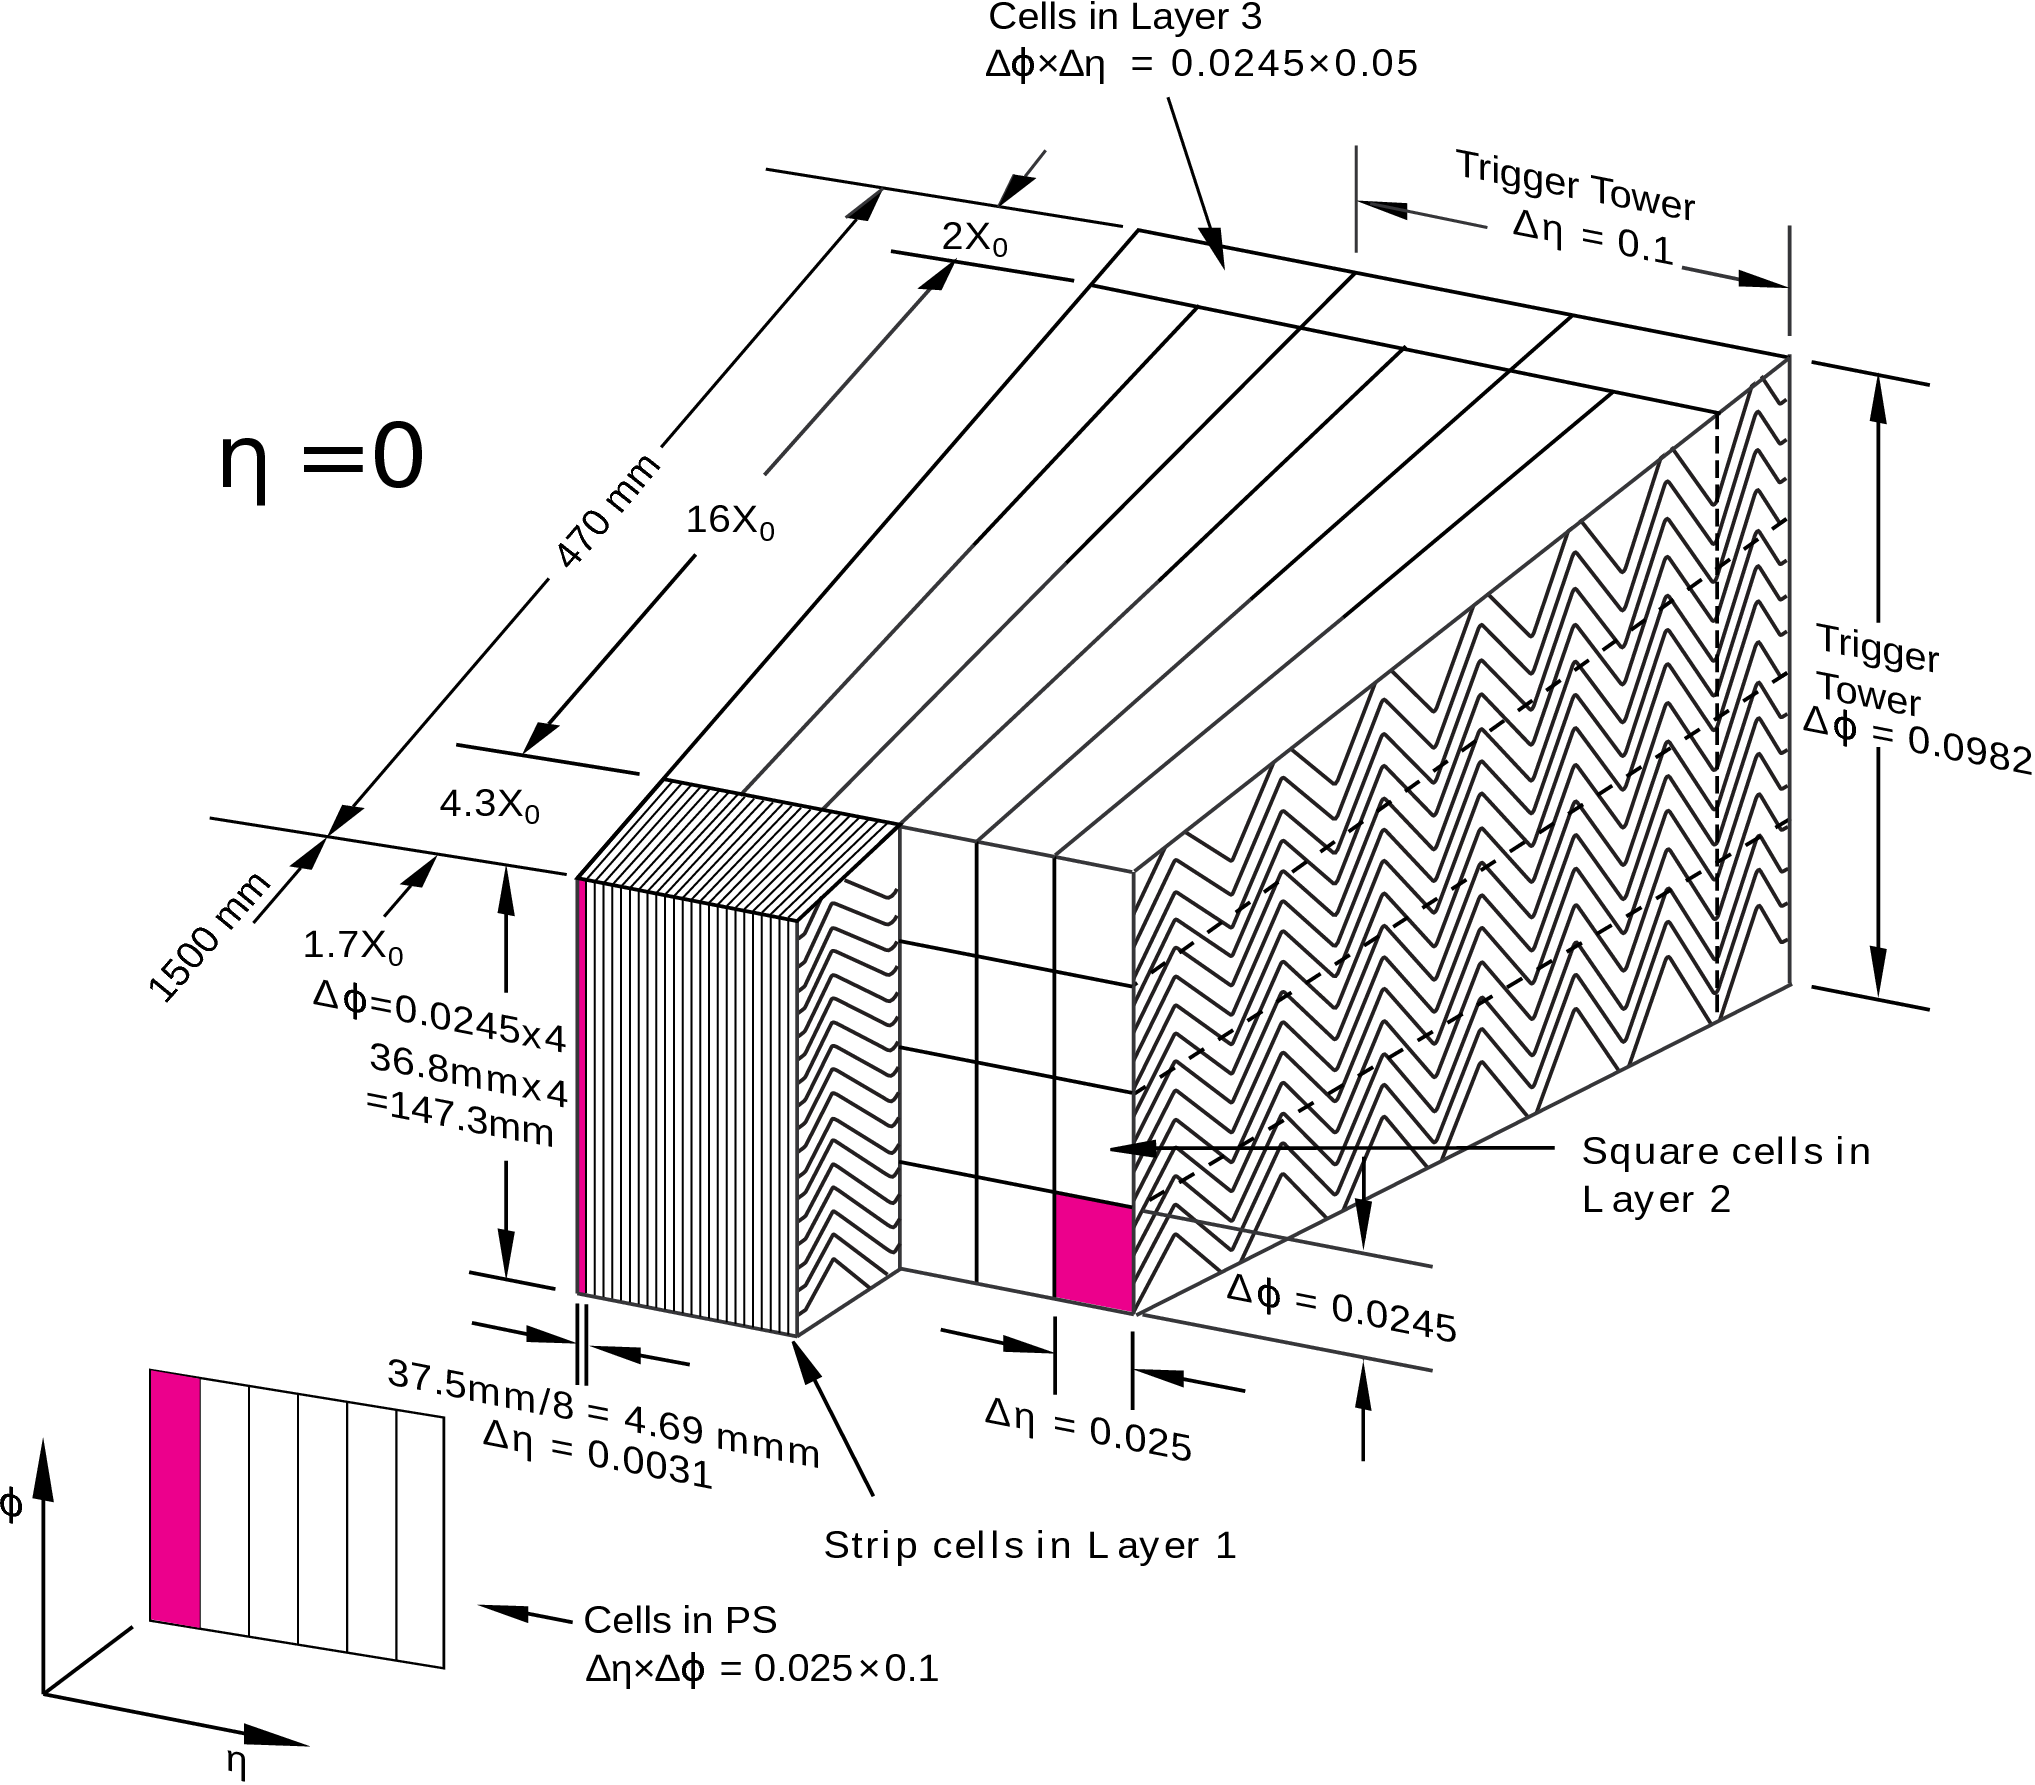
\includegraphics[width=1.\textwidth]{Part6/Img/EM.png}
\end{figure}
\column{0.6\textwidth}

\begin{itemize}
    \item \textcolor{structurColor}{\textbf{3 layers}} with different \textbf{cell size} (+ Presampler)
    \item \textbf{$N_{\eta}\times N_{\phi}$ cluster} contains most $\gamma$ energy
    \pause
    \item \textcolor{HHturquoise_d}{\textbf{Shower shapes}} (SS) quantities ($\sim$ 11) evaluated from 7$\times$11 cluster
    \begin{itemize}
        \item \textbf{Lateral} \& \textbf{longitudinal} EM shower
        \item \textbf{Discriminate between} \textcolor{HHred}{\textbf{prompt photons}} and \textcolor{HHblue}{\textbf{background photons}} (QCD jets)
    \end{itemize}
\end{itemize}
\visible<2-3>{
\begin{figure}
    \centering
    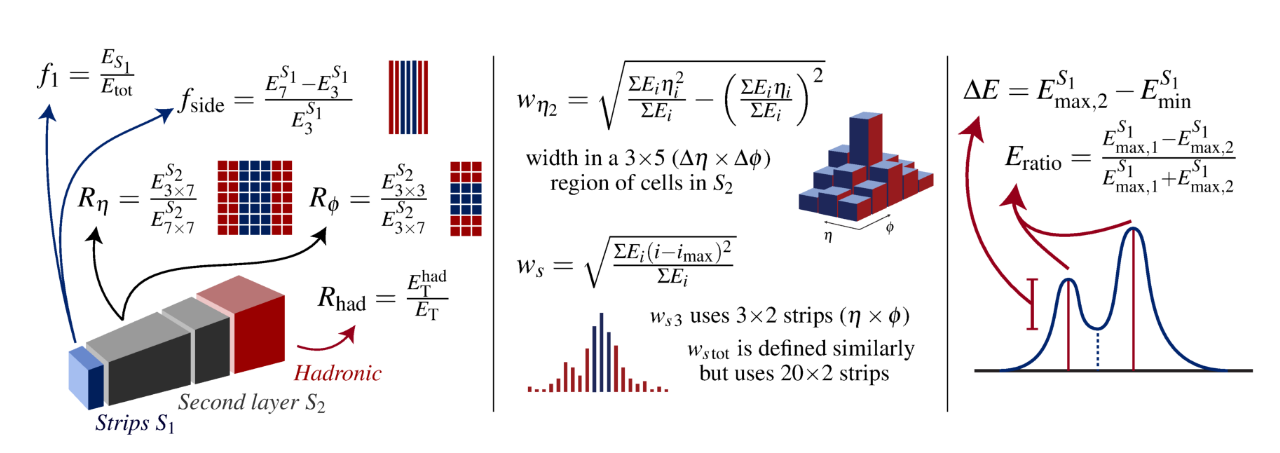
\includegraphics[width=0.8\textwidth]{Part6/Img/ShowerShapes.png}
\end{figure}
}
\pause
\begin{itemize}
    \item Current identification relies on SS: \textbf{cut-based algorithm}
    \item \textcolor{HHred}{\textbf{Propose improvement using Neural Network}}
\end{itemize}
\end{columns} 
\end{frame}

\begin{frame}{Photon identification with Neural Network}
\begin{textblock*}{5cm}(11.6cm, 7.8cm) % {block width} (coords) 
\visible<3>{
   $\eta$ direction
} 
\end{textblock*}
\begin{textblock*}{5cm}(10cm, 4.5cm)
\visible<3>{
   \rotatebox{90}{$\phi$ direction}
} 
\end{textblock*}
\begin{textblock*}{5cm}(14.5cm, 3cm) % {block width} (coords) 
\visible<3>{
   $\frac{E_{\text{cell}}}{E_{\text{cluster}}}$
} 
\end{textblock*}
\begin{columns}
\column{0.6\textwidth}    
\begin{itemize}
    \item Global shower shapes (High level) \\
    \textbf{Cut-based $\to$ DNN}
    \begin{itemize}
        \item \textcolor{HHred}{\textbf{Limited performance}} (small features space)
    \end{itemize}
    \pause
    \item Solution: \textbf{\textcolor{HHturquoise_d}{breakdown to cell level}} (Low level)
    \begin{itemize}
        \item Scale up features space dimensionality
        \begin{itemize}
            \item \textbf{Generate more variables}
            \item \textbf{Correlation between cells}
        \end{itemize} 
    \end{itemize}
    \pause
    \item \textcolor{structurColor}{\textbf{Convolutional Neural Network (CNN)}}
    \begin{itemize}
        \item Photon cluster represented as an image
    \end{itemize}
    \item Photon identification (ID) using images from the 3 layers 
\end{itemize}    
\column{0.4\textwidth}  

\visible<3>{
\begin{center}
    7$\times$11 cluster from 2$^{nd}$ layer
\end{center}
\begin{figure}
        \centering
        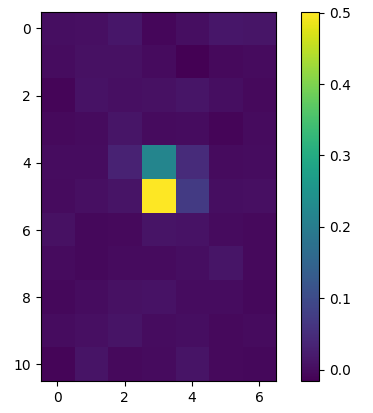
\includegraphics[width=0.8\textwidth]{Part6/Img/7_11_cluster.png}
\end{figure}
}

\end{columns}
\end{frame}

\begin{frame}{Convolutional Neural Network strategy and training}
\begin{textblock*}{5cm}(12cm,0.1cm) % {block width} (coords) 
   \textcolor{HHred}{\Large\textbf{my own work}}
\end{textblock*}
\begin{columns}
\column{0.6\textwidth}    
\begin{itemize}
    \item \textcolor{HHred}{\textbf{Prompt photons}}: inclusive $\gamma$+jets events
    \item \textcolor{HHblue}{\textbf{Background photons}}: QCD di-jet events 
    %\item + truth matching 
    \pause
    \item Images from \textbf{7$\times$11 windows} 
    \begin{itemize}
        \item \textbf{Energy independent algorithm}
        \item Image pixel = cell energy fraction
    \end{itemize}
    \pause
    \item \textbf{Inclusive training} ($E_T$, $|\eta| < $ 2.4, conversion type)
    \item \textbf{Trained on Monte Carlo}
    \end{itemize}
    \pause
    \begin{itemize}
        \item CNN \textcolor{HHred}{\textbf{over-performs}} the cut-based algorithm
    \end{itemize}
    
    
\column{0.4\textwidth} 

\begin{figure}
    \begin{overprint}
    \onslide<1-3>\centering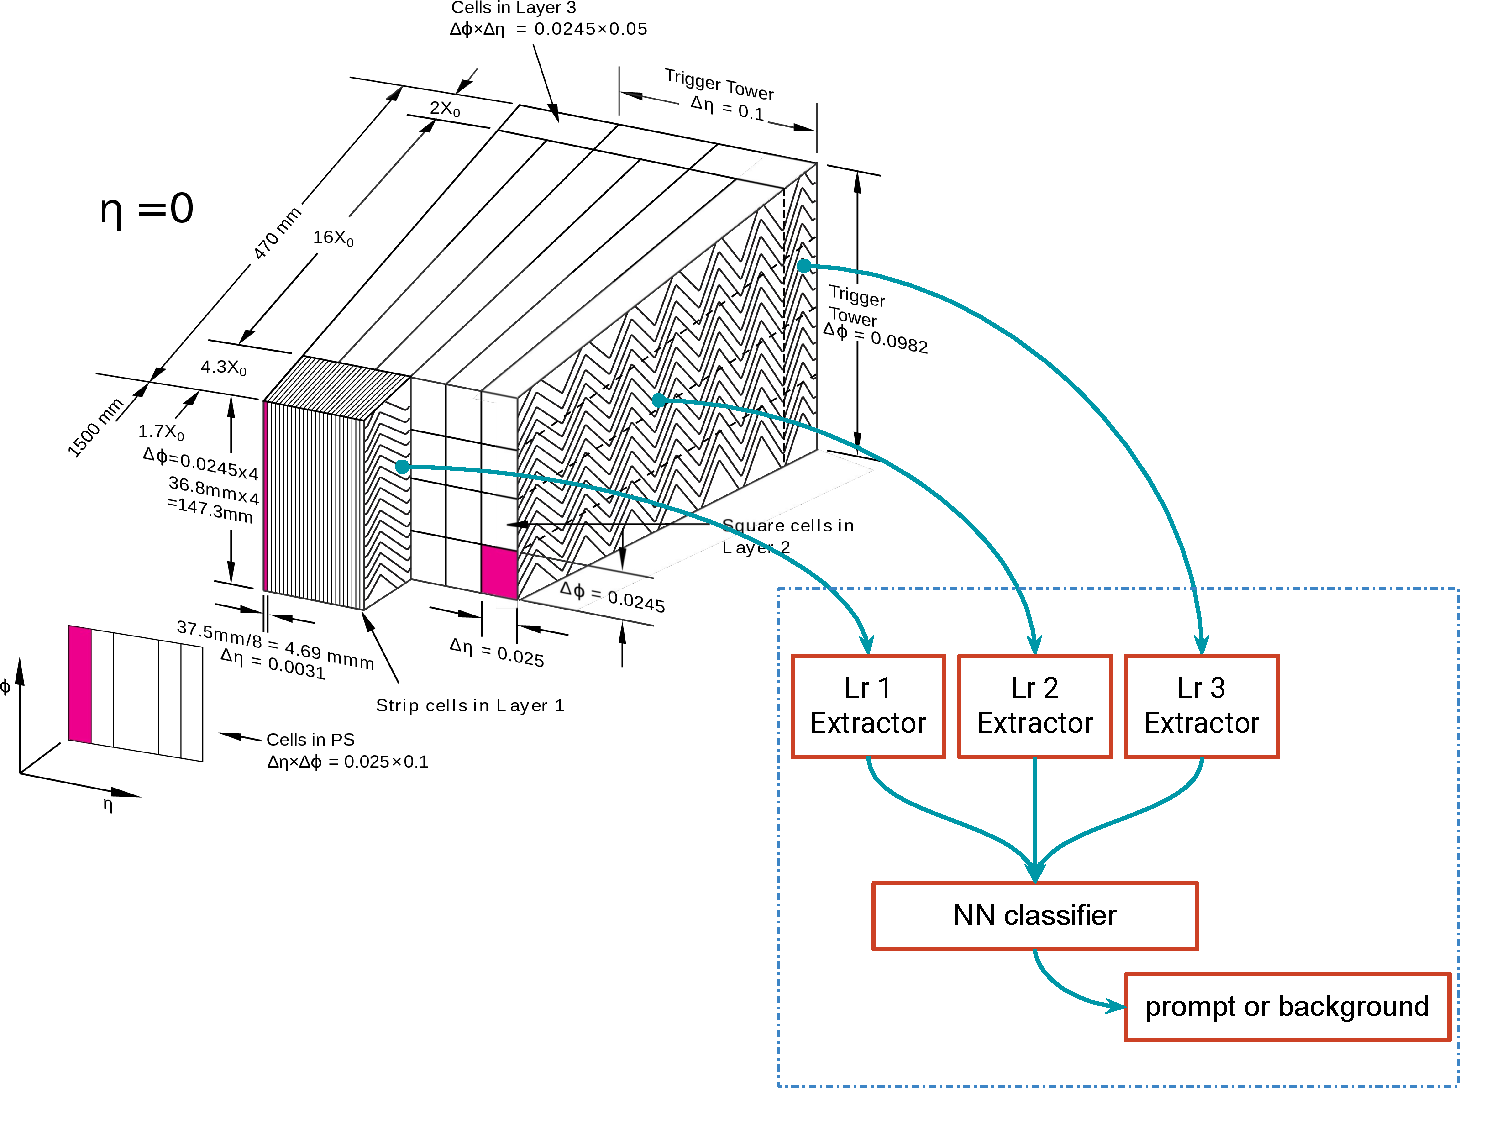
\includegraphics[width=1.1\textwidth]{Part6/Img/CNN_Idea2.pdf}
    \onslide<4>\centering\fcolorbox{HHred}{HHwhite2}{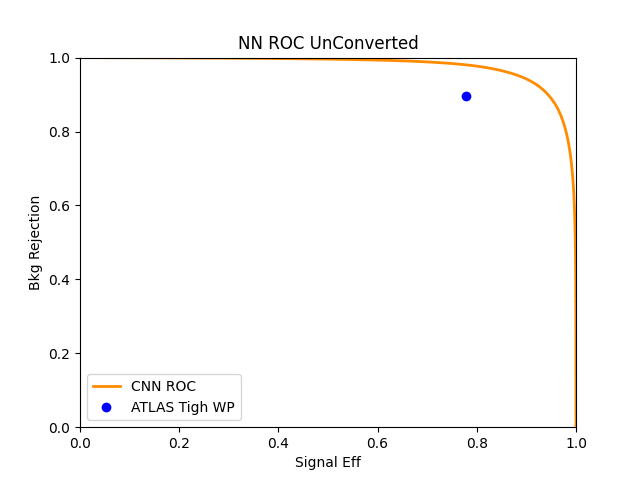
\includegraphics[width=1\textwidth]{Part6/Img/ROC_UnConverted.png}}
    \end{overprint}
\end{figure}
\end{columns}
\end{frame}

\subsection{Photon identification efficiency}
\begin{frame}{Photon identification efficiency}
\begin{textblock*}{5cm}(12cm,0.1cm) % {block width} (coords) 
   \textcolor{HHred}{\Large\textbf{my own work}}
\end{textblock*}
\begin{columns}
\column{0.6\textwidth}

\begin{itemize}
    \item Identification efficiency with \textcolor{HHred}{\textbf{Radiative Z method}} 
    \begin{itemize}
        \item Z$\to ll\gamma$ ($l$=$e$,$\mu$), \textbf{as a signal}
        \item Z$\to ll$+jet ($l$=$e$,$\mu$), \textbf{as a background}
        \item \textbf{2017 data} (43.6 fb$^{-1}$)
    \end{itemize}
    \item Efficiency as
    \begin{equation*}
        \epsilon_{ID} = \frac{N^{\text{after ID}} \times P^{\text{after ID}}}{N^{\text{before ID}} \times P^{\text{before ID}}}
    \end{equation*}
    \onslide<2->{
    \item Purity estimated with \textcolor{HHturquoise_d}{\textbf{template fit of $m_{ll\gamma}$}}
    }
    %\begin{itemize}
    %    \item signal template \textbf{from Monte Carlo}
    %    \item \textbf{second-order polynomial function} for background
    %    \item \textcolor{structurColor}{\textbf{$E_T^{\gamma} > $ 30 GeV, pure photon samples}} 
    %\end{itemize}
    \onslide<2->{
    \item \textcolor{HHred}{\textbf{Over-performs}} the cut-based algorithm
    \begin{itemize}
        \item Out-of-sample validation: \textbf{different event topology}
        \item \textbf{Good data-MC agreement}
    \end{itemize}
    }
\end{itemize}

\column{0.4\textwidth}

\begin{figure}
    \begin{overprint}
    %\onslide<2>\centering\fcolorbox{HHturquoise_d}{HHwhite2}{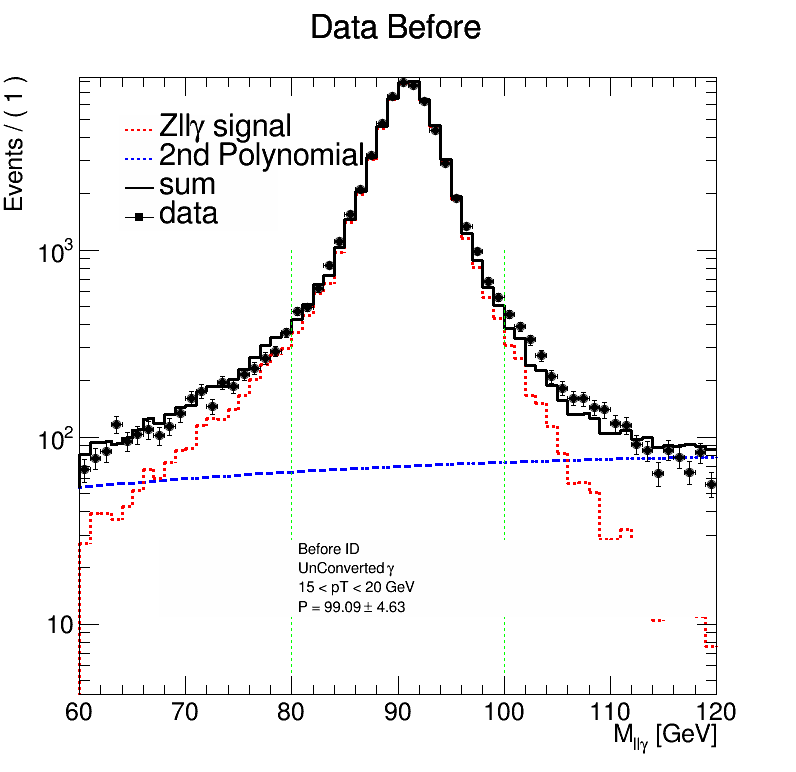
\includegraphics[width=1.\textwidth]{Part6/Img/UnConvertedllg_Before_ID_Bin_1.png}}
   % \onslide<2>\centering\fcolorbox{structurColor}{HHwhite2}{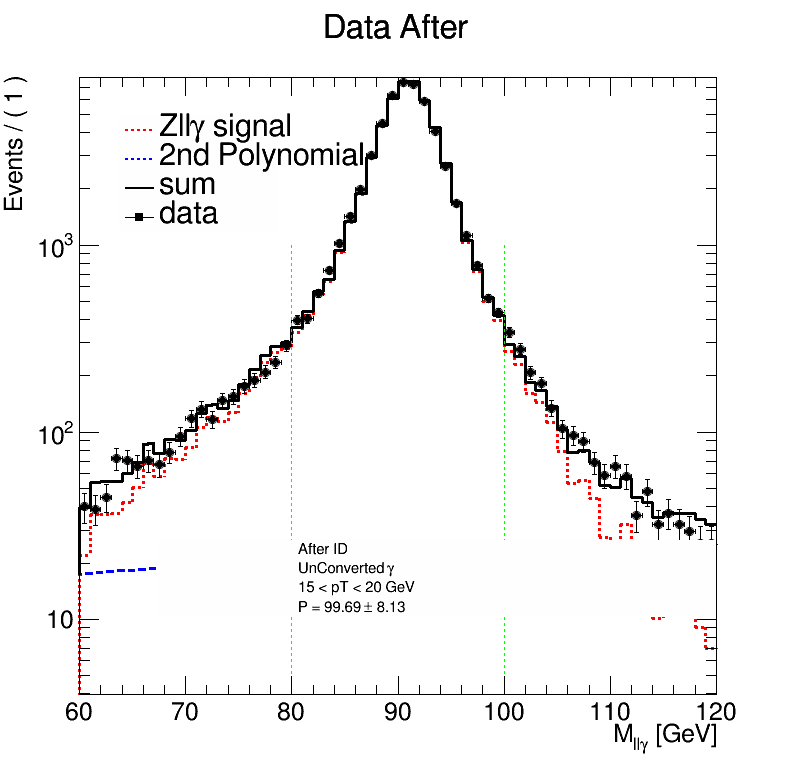
\includegraphics[width=1.\textwidth]{Part6/Img/UnConvertedllg_After_ID_Bin_1.png}}
    \onslide<2->\centering\fcolorbox{HHred}{HHwhite2}{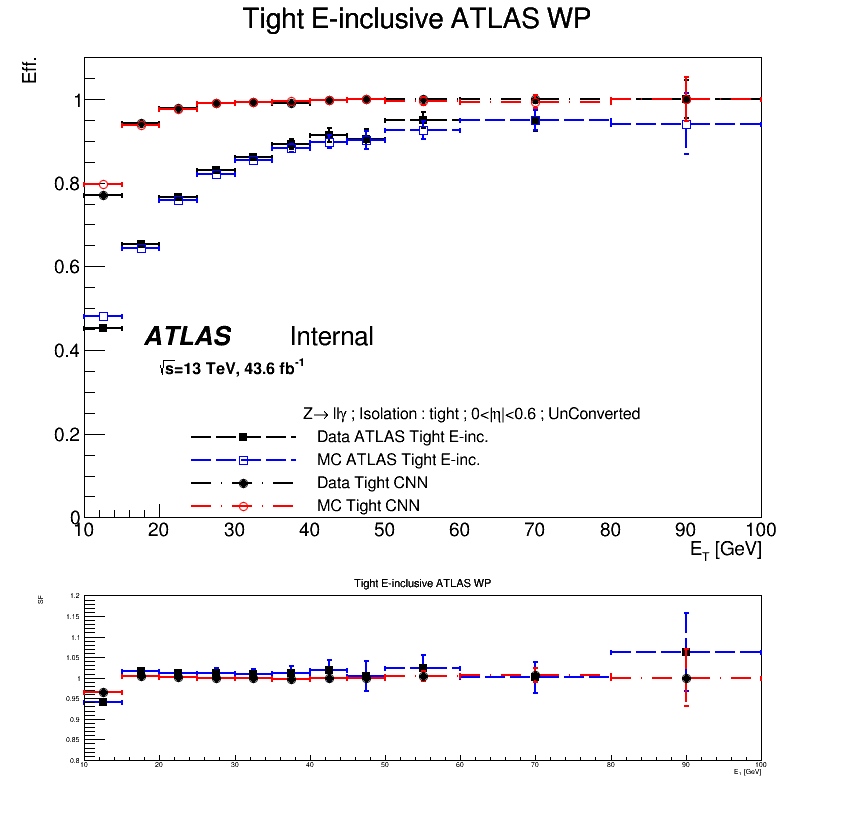
\includegraphics[width=1.\textwidth]{Part6/Img/Tight_Inc_vs_Tight_CNN__UnConverted_Iso_tight_Wgt_ETA_Bin_1.png}}
    \end{overprint}
\end{figure}

\end{columns}
\end{frame}

%\subsection{Impact on HH$\to b\bar{b}\gamma\gamma$}
\begin{frame}{Impact on HH$\to b\bar{b}\gamma\gamma$ analysis}
\begin{textblock*}{5cm}(12cm,0.1cm) % {block width} (coords) 
   \textcolor{HHred}{\Large\textbf{my own work}}
\end{textblock*}
\begin{columns}
\column{0.6\textwidth}    
\begin{itemize}
    \item CNN applied to photons from HH$\to b\bar{b}\gamma\gamma$ signal
    \begin{itemize}
   
        \item \textcolor{HHturquoise_d}{\textbf{Efficiency close to 100\%}}
    
   
        \item \textbf{15\% improvement in signal acceptance}
    
    \end{itemize}
    
    \item CNN applied to photons from continuum $\gamma\gamma$+jets
    
    \begin{itemize}
    
        \item \textcolor{HHturquoise_m}{\textbf{high $\gamma\gamma$ purity}}
        \item \textbf{15\% increase in statistics}
        \item \textbf{Reduce background modelling systematics}
    
    \end{itemize}

    \item \textbf{\textcolor{HHred}{$\sim$ 7.3\%} improvement in analysis significance}
    
    
\end{itemize}
\column{0.4\textwidth}    

\begin{figure}
    \begin{overprint}
    \onslide<1->\centering\fcolorbox{HHturquoise_d}{HHwhite2}{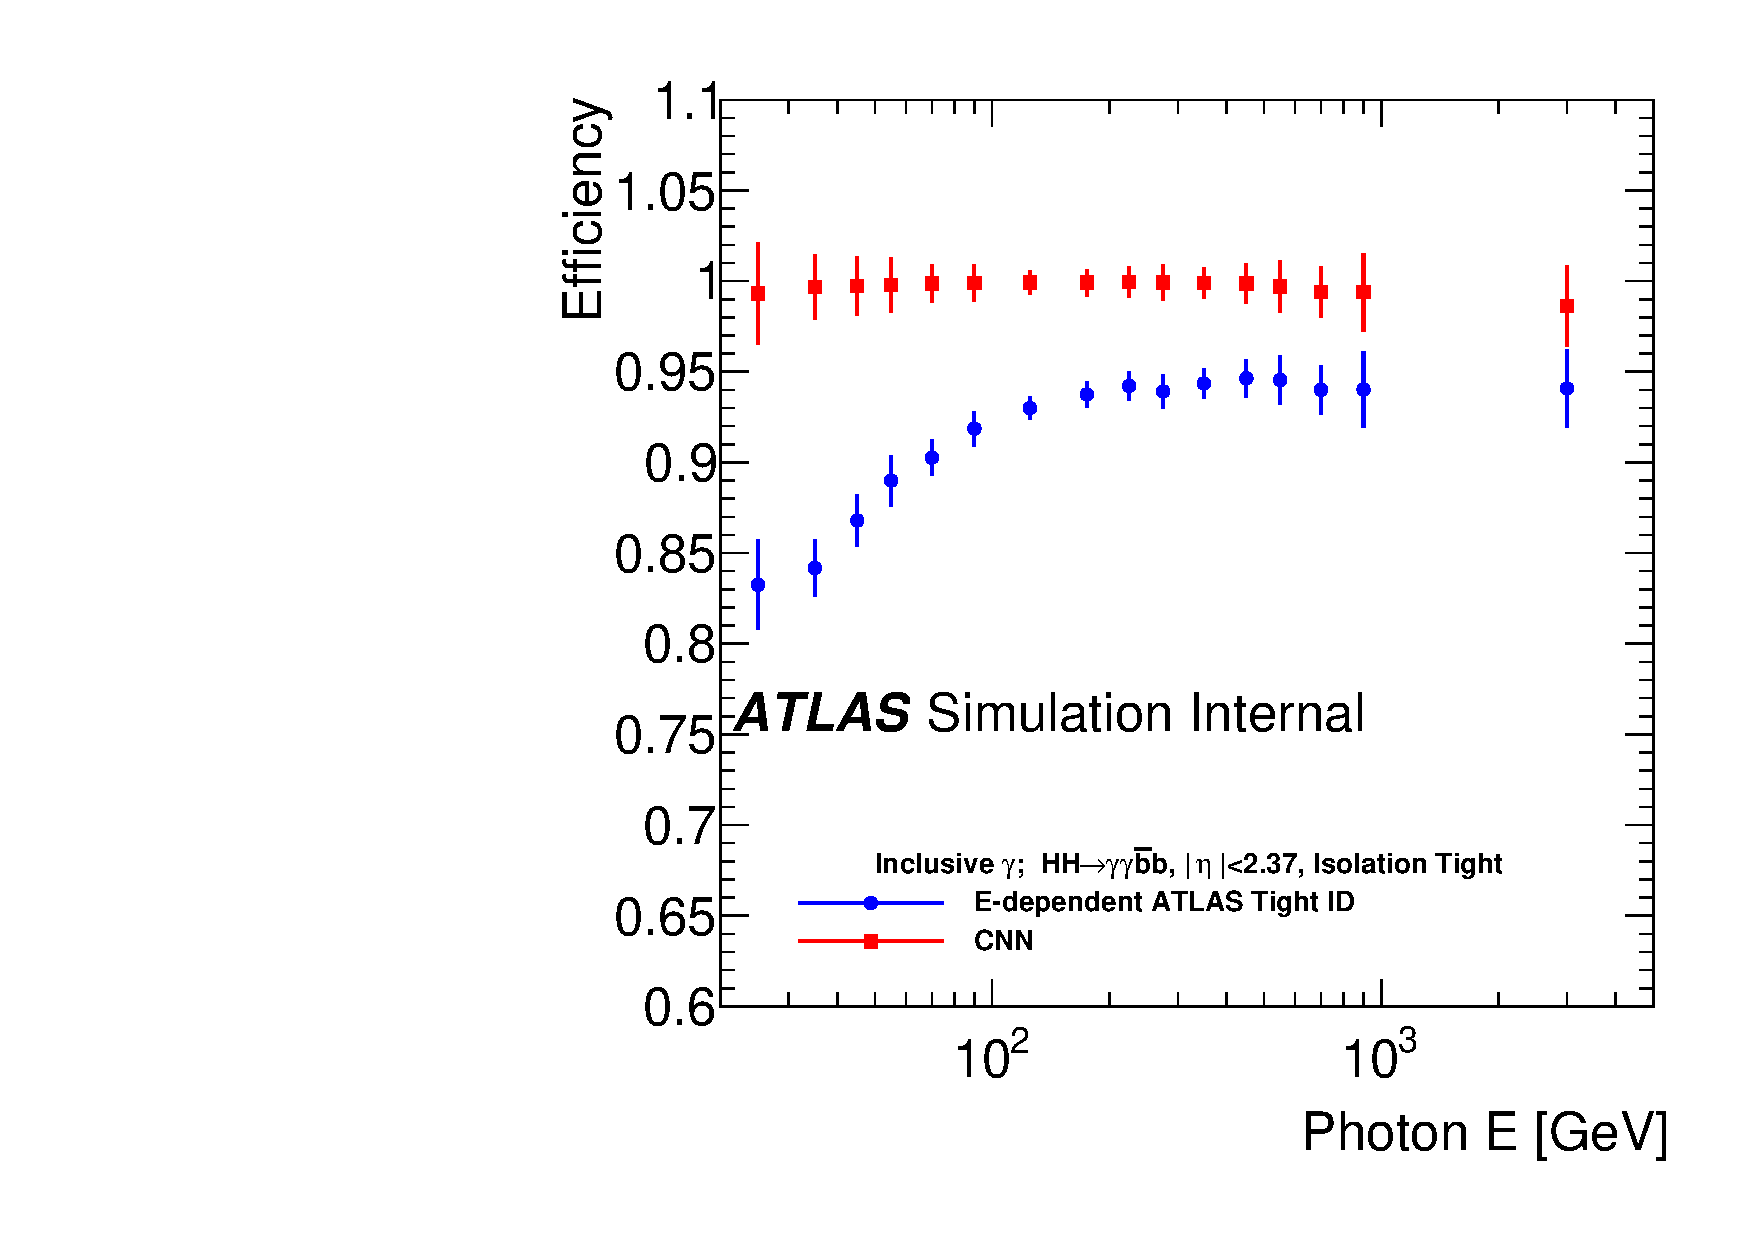
\includegraphics[width=1\textwidth]{Part6/Img/Eff_Tight_All_Inclusive_Tight_E_Sig.pdf}}
   % \onslide<3>\centering\fcolorbox{HHturquoise_d}{HHwhite2}{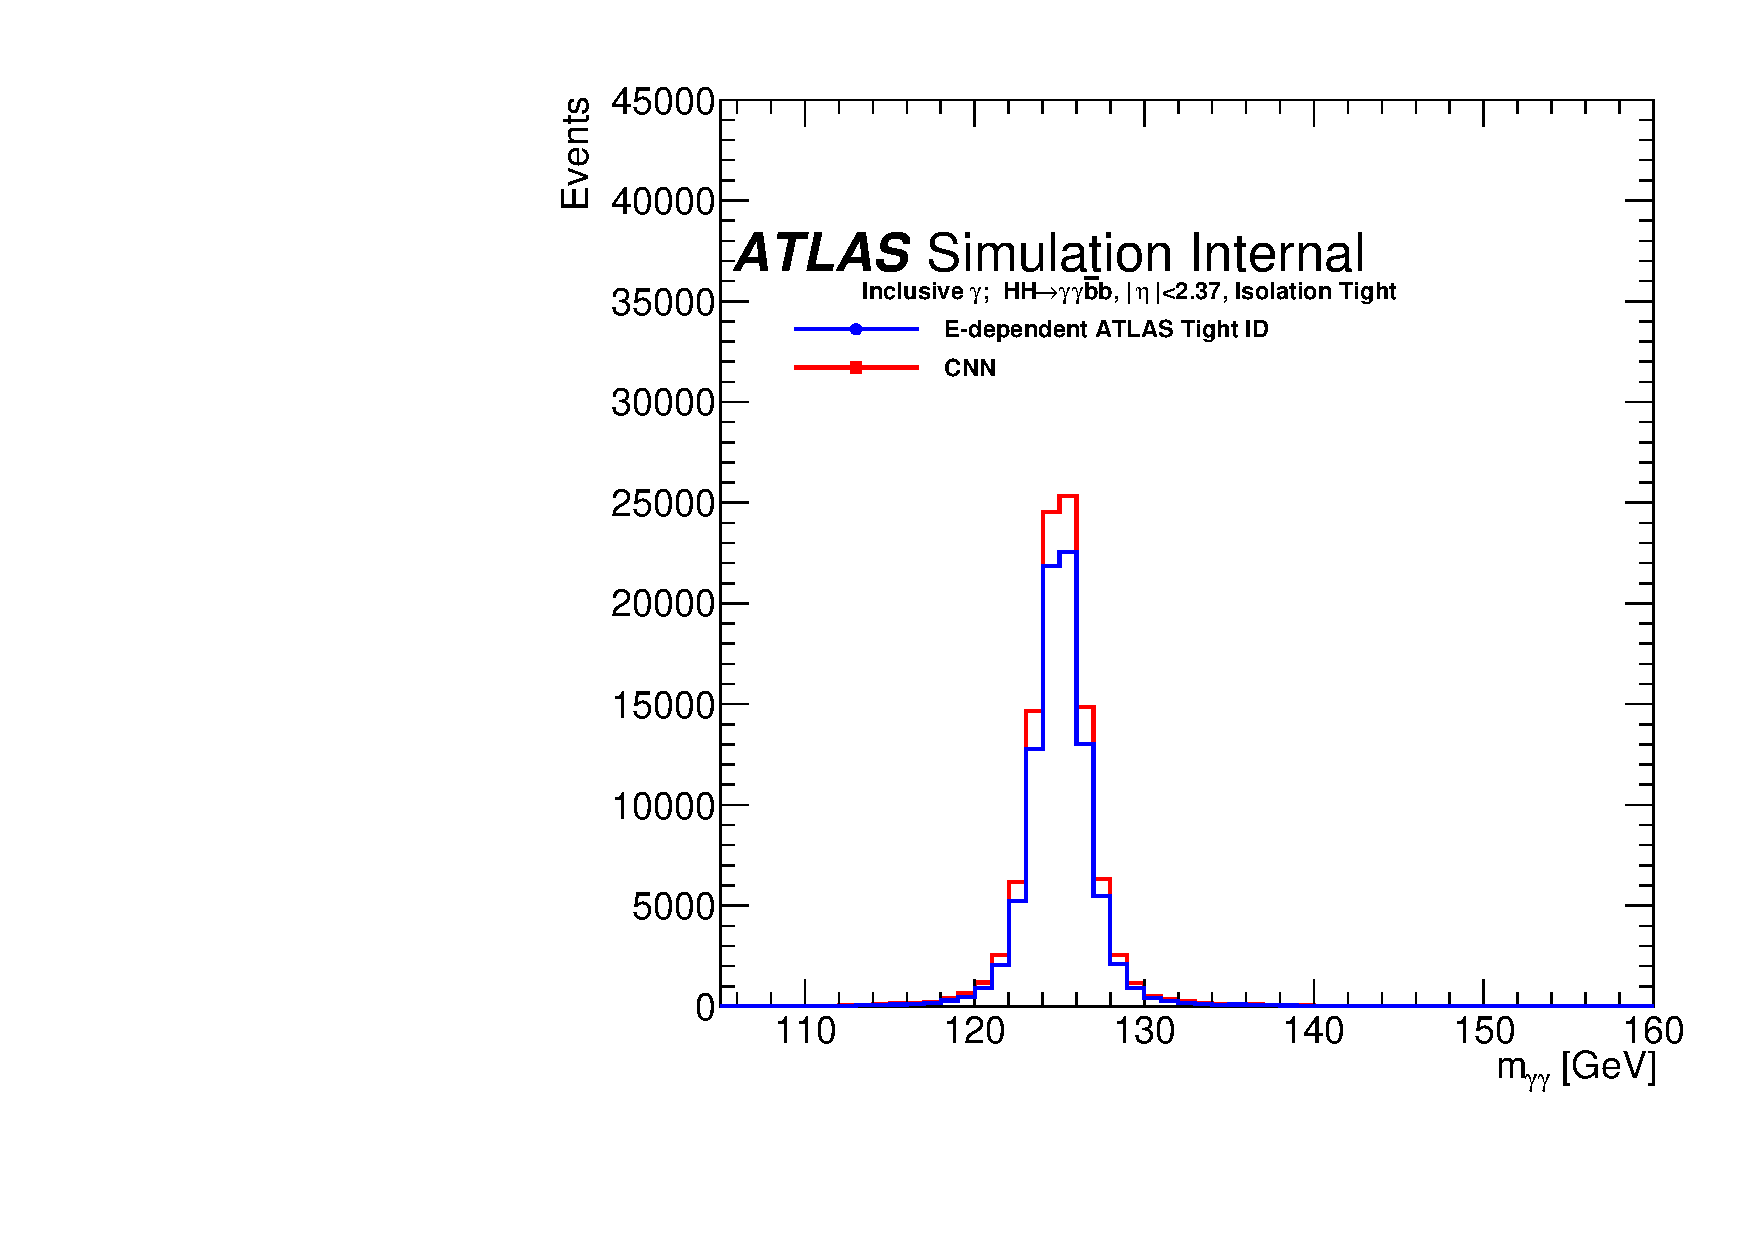
\includegraphics[width=1\textwidth]{Part6/Img/Eff_Tight_All_Inclusive_Tight_M_Sig.pdf}}
    %\onslide<5>\centering\fcolorbox{HHturquoise_m}{HHwhite2}{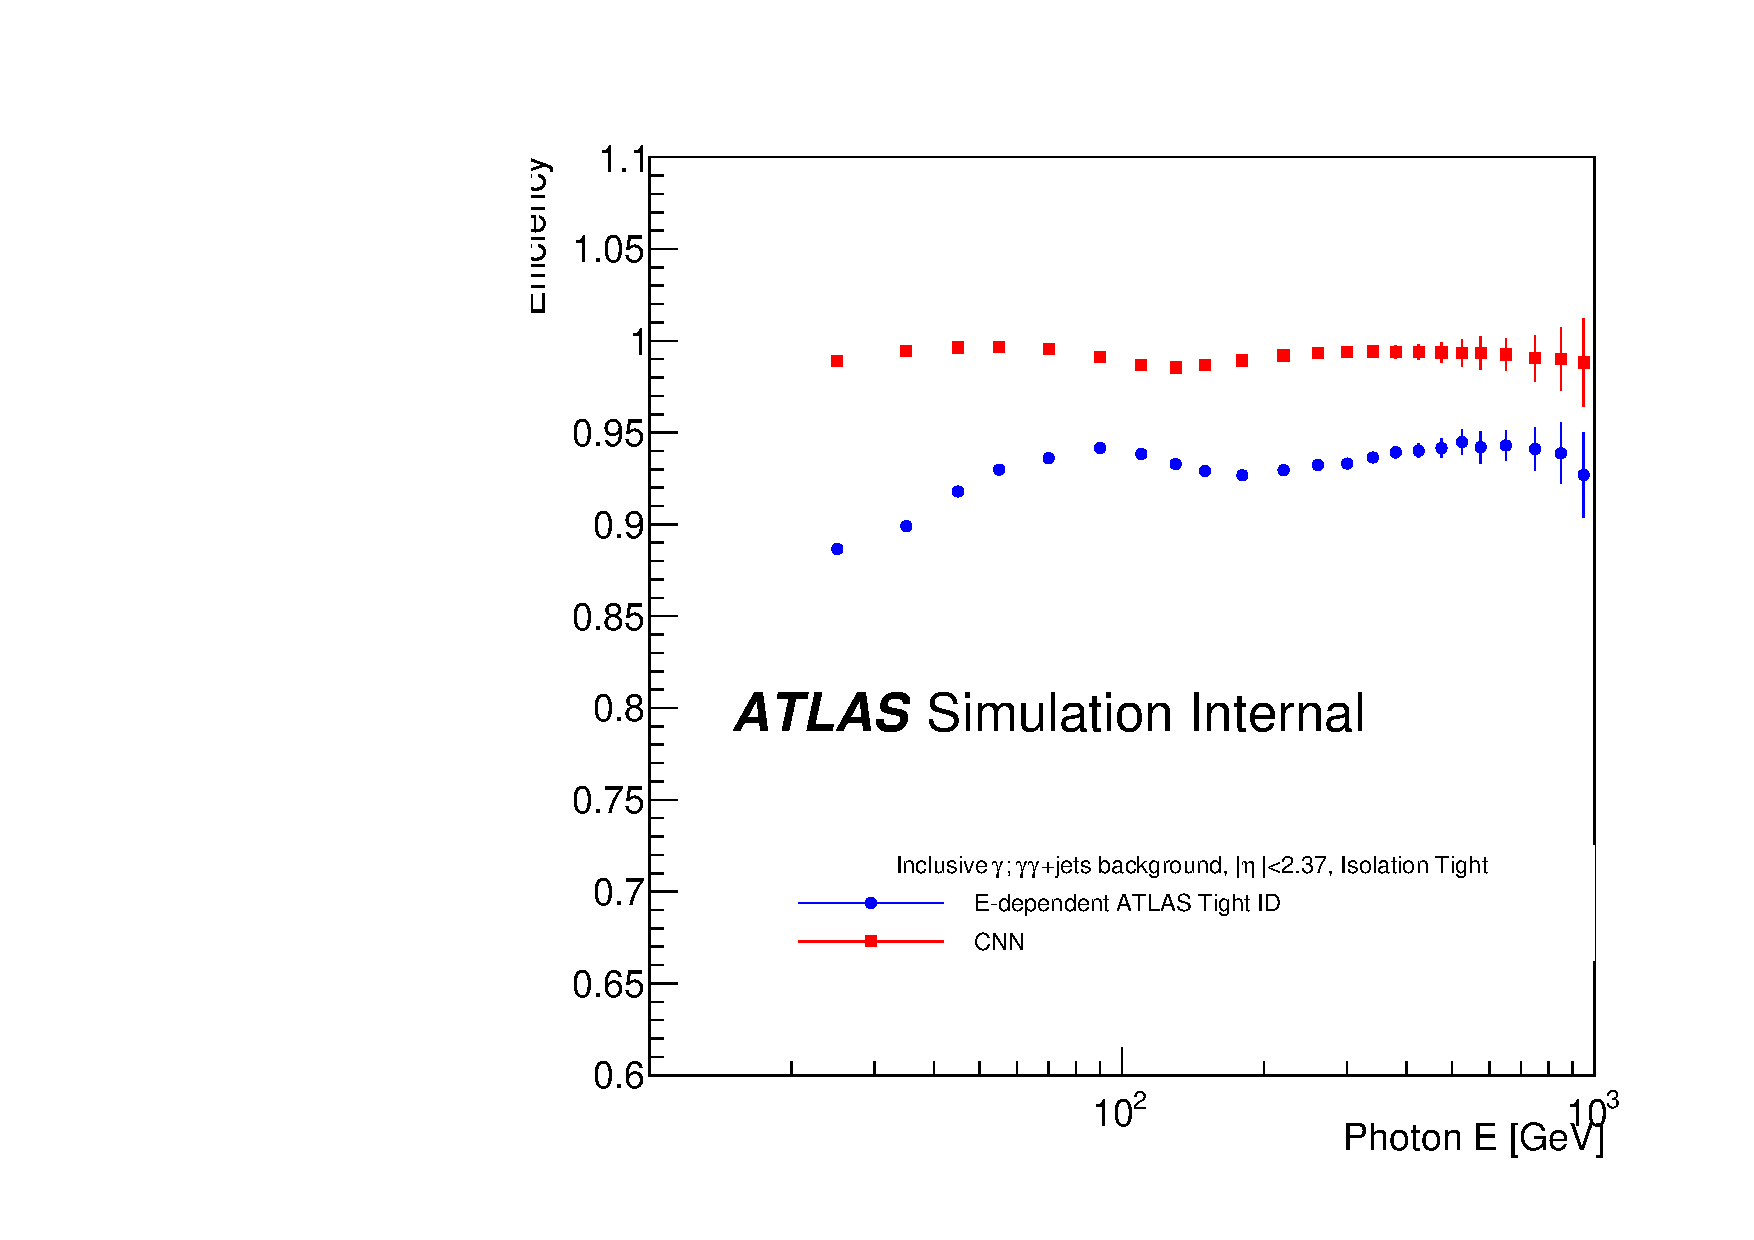
\includegraphics[width=1\textwidth]{Part6/Img/Eff_Tight_All_Inclusive_Tight_E_Bkg.pdf}}
    %\onslide<6>\centering\fcolorbox{HHturquoise_m}{HHwhite2}{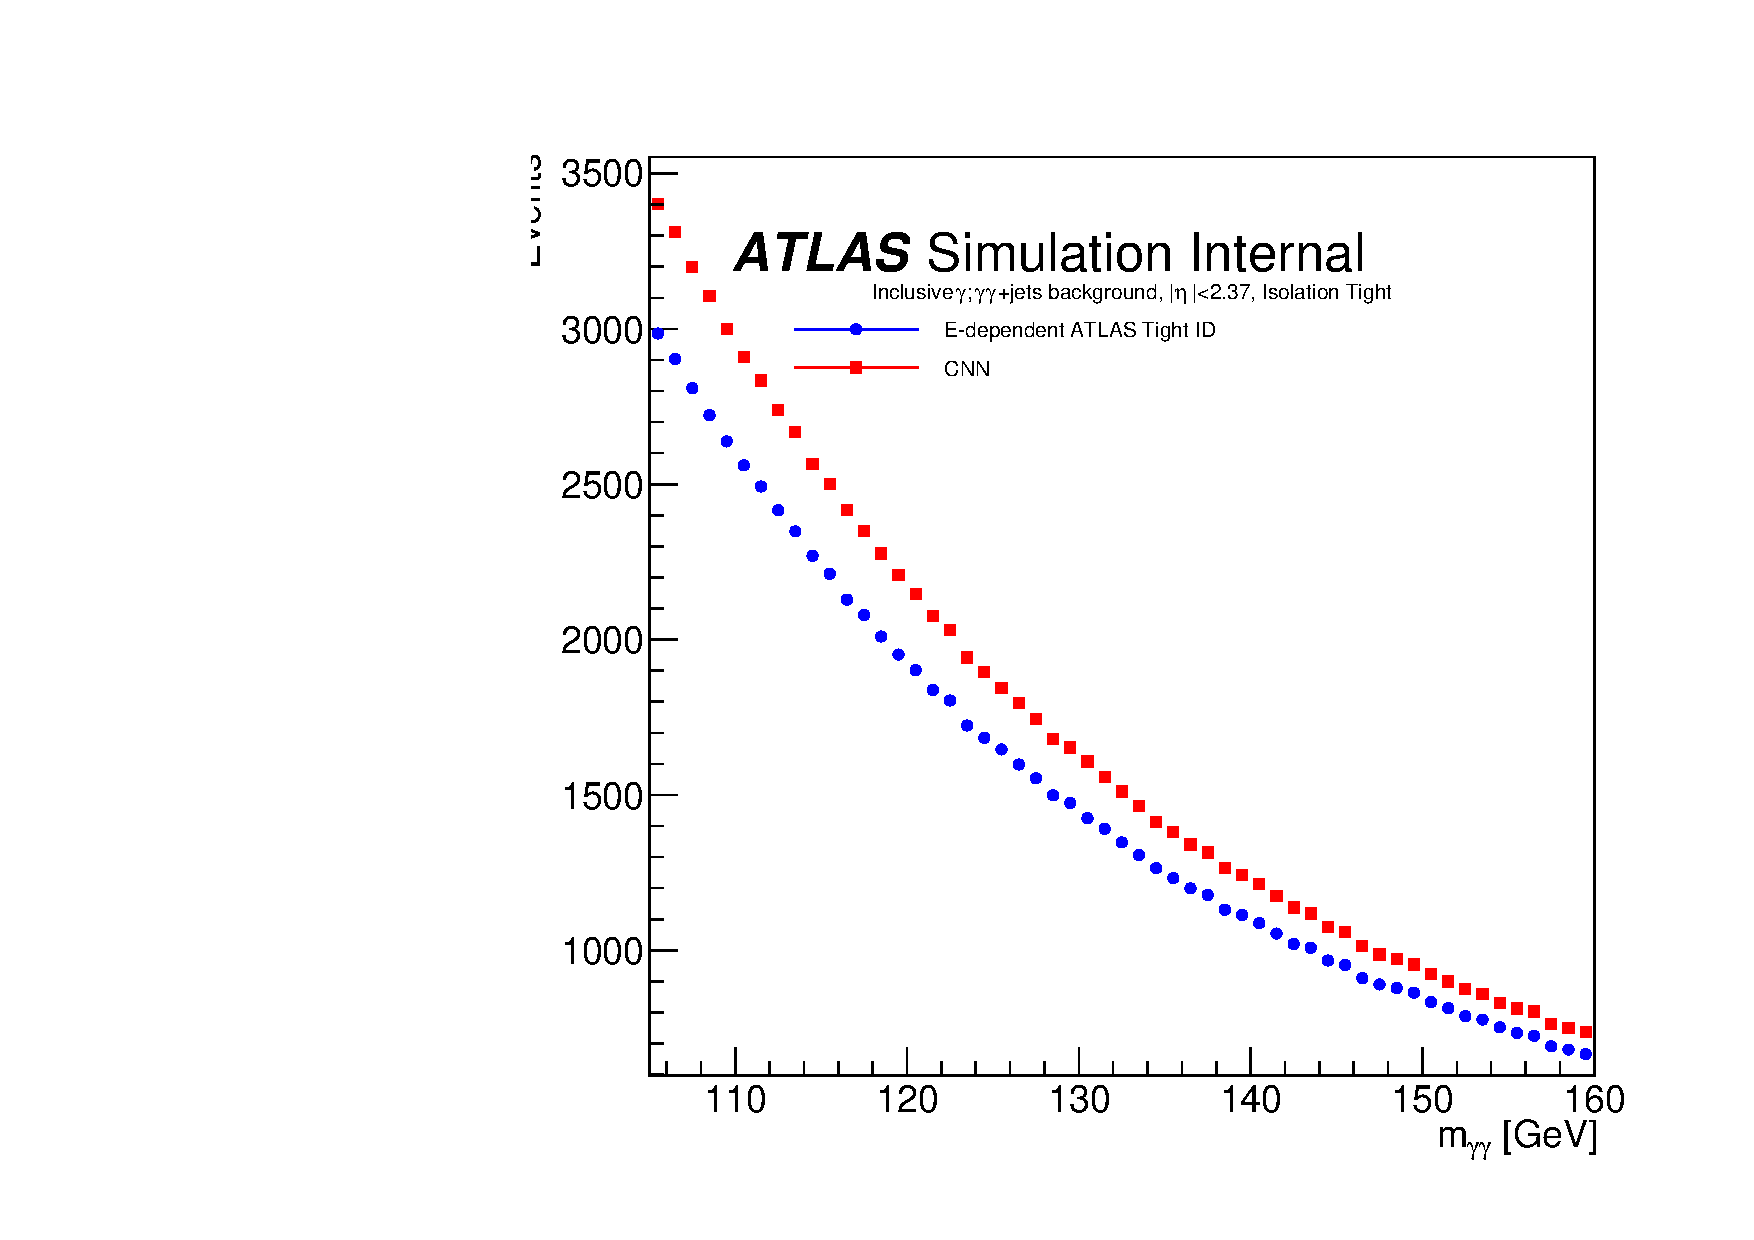
\includegraphics[width=1\textwidth]{Part6/Img/Eff_Tight_All_Inclusive_Tight_M_Bkg.pdf}}
    \end{overprint}
\end{figure}
\end{columns}

\end{frame}

%\subsection{Future improvement}
%\begin{frame}{Future improvement}
%    \textbf{Is really needed}
%\end{frame}